\chapter{Répartition des sources de production d'énergies}
% \section{}
% \section{Réutilisation des sources de chaleur}

L'emplacement des points de production sont importants dans la lutte contre le gaspillage énergétique.
Plusieurs points importants entrent en ligne de compte, comme le coût du transport de cette énergie ainsi que les pertes liées à ce mode de transport.
Peu importe la technologie utilisée, les lois de la thermodynamique rendent impossible le transport gratuit d'énergie.

\section{Perte d'énergie en chaleur}

Prenant en compte la 1ère loi de la thermodynamique, lors de toute transformation, il y a
conservation de l'énergie.
Ainsi, dans un espace clos, l'énergie ne peut varier.
Prenons pour espace le câble qui fait transiter l'énergie de la production à la consommation.

Le transport de l'énergie va transformer en chaleur une partie de celle-ci en raison
des forces de frottement des électrons sur les atomes.

Il est possible de réduire cette perte en utilisant des matériaux plus conducteurs que
d'autres, mais il n'est pas possible de l'annuler.
De plus, pour des raisons économiques, ces matériaux supraconducteurs ne peuvent être
déployés en masse du fait de leur coût, et des conditions nécessaires à leur stabilité.
Le Diborure de magnésium $MgB_2$ est un des matériaux ayant la plus haute température
critique avec 39 K (-234 C).

Aujourd'hui, la majorité des câbles électriques mondiaux sont en cuivre ou en aluminium.
Nous nous intéresserons plus particulièrement au cuivre qui possède le meilleur rendement.

Pour calculer la perte d'énergie dans un câble en cuivre, on peut utiliser
la formule $Loss = I^2\times R$ avec $I$ pour l'intensité, exprimée en ampère, et $R$ en Ohm.

On peut exprimer les Ohms avec la formule suivante : $R = \frac{V}{I_r}$
avec $V$ pour le voltage et $I_r$ pour l'intensité perdue par la résistance du matériaux.

Cette formule montre que augmenter l'intensité augmente beaucoup plus la perte d'énergie
que le voltage.

Cette relation explique pourquoi il est plus rentable de créer des lignes à haute tension
pour de longues distances.
Cependant, un voltage élevé amène d'autres problèmes comme un électromagnétisme intense,
c'est pourquoi les lignes à haute tensions sont en haut de grand pilonnes.

C'est l'entreprise RTE qui décide en France du voltage et fait ce choix pour minimiser les coûts de
fabrication et limiter les pertes d'énergie.

En comparaison, les lignes électriques du Canada ou des États-Unis utilisent un voltage
plus important car les distances que parcoure l'énergie est plus conséquente.

En France, on utilise la norme \texttt{NF\_C18-510} pour classer les lignes électriques.

\begin{table}[h]
  \begin{tabular}{|l|l|l|}
    Tension    & Courent Alternatif     & Courent Continue        \\
    Très basse & $U_n \leq 50V$         & $U_n \leq 120V$         \\
    Basse      & $50V < U_n \leq 1kV$   & $120V < U_n \leq 1.5kV$ \\
    Haute      & $1kV < U_n \leq 50kV$  & $1.5kV < U_n \leq 75kV$ \\
    Très Haute & $U_n > 50kV$           & $U_n > 75kV$            \\
  \end{tabular}
\end{table}

Chacune de ces tensions sont utilisées pour des besoins spécifiques.

Le courant alternatif est plus utilisé car il chauffe moins les ligne électriques,
et pert moins d'énergie.

\section{Topologie et répartition}

Les méthodes de production et de distributions d'énergies sont en train de changer en réponse
à la diversification des moyens de production.

Avec des consommateurs pouvant générer de l'électricité sur leurs toits, ou dans leurs jardin,
ceux-ci deviennent ce que l'on appelle en anglais des \textit{prosumer}.
Ce mot est issu de la contraction des mots \textit{producer} (producteur) et
\textit{consumer} (consommateur).

Dans le futur de la distribution, tout les nœuds du réseau seront susceptibles de produire de l'énergie.
Il s'agit donc d'une distribution bi-directionnelle.

De nombreux défis existent pour concevoir cette transformation, dont ceux déjà évoqués un peu plus tôt dans ce papier.
Cependant il reste un problème de taille pour clôturer ce chapitre.

Comment faire évoluer un réseau existant à bas voltage pour faciliter la mise en œuvre des technologies
de Smart Grid ?

La topologie est un outil mathématique adéquat pour répondre à ces problématiques d'optimisation
et de partage de l'information avec ces nœuds.
Prenons le graphe \ref{fig:ieee_radial_tree} représentant topologiquement un arbre,
puisqu'il s'agit du format traditionnel de représentation des réseaux de distribution.
Les \textit{prosumer} sont représentées par les nœuds du graphe,
tandis que les lignes électriques sont représentées par les arcs entre les nœuds.

La première remarque du système actuel est que la distribution d'énergie contribue de 8 à 15\% de perte
d'énergie en chaleur.

Dans le schema \ref{fig:ieee_radial_tree}, le symbole du nœud 799 est un transformateur qui
fonctionne en tant qu'interrupteur tandis que le symbole entre les nœuds
709 et 775 est un transformateur qui contrôle le voltage.

\begin{SCfigure}[2][h]
  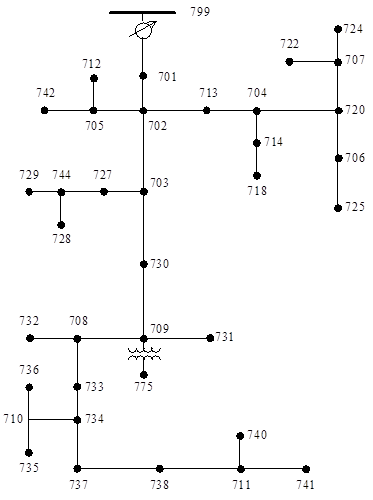
\includegraphics[scale=0.5]{media/ieee_radial_tree.png}
  \caption{
      IEEE 37 nœuds de test\newline
      \tiny{Source:\newline
        Smart Grid Topology Designs
      }
  }
  \label{fig:ieee_radial_tree}
\end{SCfigure}

Considérons un réseau de distribution d'électricité basse tension existant dans une zone urbaine modélisée,
$G = (N, A)$ pour un ensemble de $n$ nœud $N = \lbrace 1 \dots, n \rbrace$ de sorte que la topologie soit un arbre enraciné
au nœud $n_0$, soit le nœud 799 du schéma. $A$ représente l'ensemble des arcs, à savoir les câbles du réseau.

Historiquement, l'électricité devait être fournie par le contrôleur (en France RTE) en réponse à la demande des consommateurs,
de sorte que les graphes étaient considérés comme orientés.
Nous faisons quelques hypothèses pour simplifier le traitement du flux de courant alternatif non linéaire.

Considérons que l'ensemble $N \backslash n_0$ est divisé en un ensemble $C$ des utilisateurs finaux qui restent des consommateurs et
en un ensemble $P$ des nouveaux \textit{prosumer}.

L'électricité peut être renvoyée par le \textit{prosumer} dans le réseau de distribution sans qu'il soit nécessaire
de créer des arcs supplémentaires, et elle peut être contrôlée et surveillée par des dispositifs de commutation.
On peut donc supposer que le réseau existant est modélisé par $\bar{G} = (N, E)$

Considérant une horizon temporelle $T$,
tous les utilisateurs $i \in N \backslash n_0$ consomment une quantité
$EC^t_i$ d'énergie à un temps $t$.
Tous les \textit{prosumer} $i \in P$ génèrent une quantité
$EG^t_i$ d'énergie à un temps $t$.

À chaque unité de temps $t$ l'énergie demandé est de $Q^t_i$ pour chaque consommateur
$i \in C$ tel que $Q^t_i = -EC^t_i$.

À chaque unité de temps $t$ l'énergie demandé est de $Q^t_i$ pour chaque \textit{prosumer}
$i \in P$ tel que $Q^t_i = EG^t_i - EC^t_i$, c'est à dire l'énergie utilisée retranchée à l'énergie produite.

\begin{itemize}
  \item Si $Q^t_i = 0$, alors le \textit{prosumer} est auto-suffisant, il ne nécessite
    ni d'export d'énergie, ni d'import.
  \item Si $Q^t_i > 0$, alors le \textit{prosumer} a un excès d'énergie, il devra en vendre.
  \item Si $Q^t_i < 0$, alors le \textit{prosumer} a un déficit d'énergie, il devra en acheter.
\end{itemize}

Le réseau est capable de transferer de l'énergie à ses voisins.
\begin{itemize}
  \item Si la somme de l'énergie demandée par les nœuds fils de $n_0$ est positive, il y a trop d'énergie. Il faut en vendre.
    Notons cette condition $\sum_{i \in N \backslash \lbrace n_0 \rbrace} Q^t_i > 0$
  \item A contrario, si cette somme est négative, il n'y en a pas suffisamment. Il faut en acheter.
    Notons cette condition $\sum_{i \in N \backslash \lbrace n_0 \rbrace} Q^t_i < 0$
\end{itemize}

Pour plus de clarté, redéfinissons $Q^t_{n_0} = \sum_{i \in N \backslash \lbrace n_0 \rbrace} Q^t_i$

La limite de l'efficacité du réseau est connue.
Cette contrainte est le maximum qu'une ligne électrique est en mesure de transporter.
Notons ce maximum $\bar{Q}$.

\begin{equation*}
  \bar{Q} = \max_{t \in T} \sum_{i \in N \backslash \lbrace n_0 \rbrace} \lvert Q^t_i \rvert
\end{equation*}


Nous remarquerons que cette valeur ne peut être négative, contrairement à nos précédentes remarques.
Il faut prendre en compte le fait que l'éléctricité ne peut circuler dans les deux sens dans un même câble.
Deux points dans le réseau seront reliés par deux câbles différents afin de pouvoir transférer l'énergie dans les deux sens.
Il s'agit d'une connexion en duplex.

On prend en compte la perte d'énergie en tant que "Loss factor" $L \in \lbrack 8, 15 \rbrack \%$

La topologie des variables $x_{ij}$ indiquent l'arc $(i, j)$ sélectionné. Il s'agit d'un de nos câble électrique.
La quantité d'énergie transportée dans ce câble entre les points $i$ et $j$ pour un temps $t$ est notée $y^t_{ij}$.

Une sécurité nous permet de nous assurer que tous les points fassent partis du réseau.
Pour se faire, nous donnons un poids $a_{ij}$ aux câbles.
Ce poids est de 1 si la câble existe dans le réseau de distribution.
Autrement il est de 0.

Pour remédier à cette absence de câble, nous prenons en compte son coût d'installation dans le calcul.
Notons ce coût $c_{ij}$, $ij \in A$.

$Eq$ est la fonction objectif \ref{prosumer_1} qui minimise le coût d'ajout de nouveaux câbles
ainsi que la perte d'énergie.

\begin{equation} \label{prosumer_1}
  Eq = \min \sum_{(i, j) \in A} c_{ij} x_{ij} + \sum_{t \in T} \sum_{(i,j) \in A} y^t_{ij}
\end{equation}

Sujet à

\begin{subequations}
  \begin{equation} \label{prosumer_2}
    \sum_{i \in N} (a_{ij} + x_{ij}) \ge 1
    \quad \quad
    j \in C
  \end{equation}
  \begin{equation} \label{prosumer_3}
    \sum_{i \in N} (a_{ij} + x_{ij}) \ge 1
    \quad \quad
    j \in P
  \end{equation}
  \begin{equation} \label{prosumer_4}
    \sum_{i \in N} (a_{ij} + x_{ij}) \ge 1
    \quad \quad
    j \in P
  \end{equation}
  \begin{equation} \label{prosumer_5}
    \sum_{i \in N} y^t_{ij} + (1 + L) Q^t_j = \sum_{i \in N} y^t_{ij}
    \quad \quad
    j \in N, t \in T
  \end{equation}
  \begin{equation} \label{prosumer_6}
    y^t_{ij} \le \bar{Q}(a_{ij} + x_{ij})
    \quad \quad
    (i, j) \in A
  \end{equation}
  \begin{equation} \label{prosumer_7}
    a_{ij} + x_{ij} + a_{ji} + x_{ji} \le 1
    \quad \quad
    i, j \in N
  \end{equation}
  \begin{equation} \label{prosumer_8}
    x_{ij} \in \lbrace 0, 1 \rbrace
    \quad \quad
    (i,j) \in A
  \end{equation}
  \begin{equation} \label{prosumer_9}
    y^t_{ij} \ge 0
    \quad \quad
    (i,j) \in A, i \in T
  \end{equation}
\end{subequations}

% \begin{subequations}
%   \begin{align}%{4}
%     E_{11} & \!\begin{aligned}[t] & = Q_{11}^2\ln\sqrt{B'_{11}} +Q_{12}^2\ln\sqrt{B'_{22}}+Q_{13}^2\ln\sqrt{B'_{33}} \\
%     &=Q_{11}^2\ln\sqrt{B'_{11}}+Q_{21}^2\ln\sqrt{B'_{33}}
%     \end{aligned}\\[0.75ex]
%     E_{12} & \!\begin{aligned}[t] & =Q_{11}Q_{21}\ln\sqrt{B'_{11}} +Q_{12}Q_{22}\ln\sqrt{B'_{22}}+Q_{13}Q_{23}\ln\sqrt{B'_{33}} \\
%     & =Q_{11}Q_{21}\ln\sqrt{B'_{11}}-Q_{11}Q_{21}\ln\sqrt{B'_{33}}
%     \end{aligned}\\[0.75ex]
%     E_{22} & \!\begin{aligned}[t] & =Q_{21}^2\ln\sqrt{B'_{11}} +Q_{22}^2\ln\sqrt{B'_{22}}+Q_{23}^2\ln\sqrt{B'_{33}} \\
%     &=Q_{21}^2\ln\sqrt{B'_{11}} +Q_{11}^2\ln\sqrt{B'_{33}}
%     \end{aligned}\\[0.85ex]
%     E_{33} & \!\begin{aligned}[t] & =Q_{31}^2\ln\sqrt{B'_{11}} +Q_{32}^2\ln\sqrt{B'_{22}}+Q_{33}^2\ln\sqrt{B'_{33}} \\
%     &=Q_{32}^2\ln\sqrt{B'_{22}}
%     \end{aligned}
%   \end{align}
%   \label{straincomponent}
% \end{subequations}



% 2
L'inégalité \ref{prosumer_2} s'assure que chaque consommateur reste connecté au réseau principal.
% 3 et 4
Les inégalités \ref{prosumer_3} et \ref{prosumer_4} s'assurent que chaque \textit{prosumer} reste connecté au réseau principal.
Vu que chaque \textit{prosumer} a la capacité de recevoir et de donner de l'énergie, la vérification
est fait en duplex.
% 5
L'égalité \ref{prosumer_5} est une contrainte de conservation de l'énergie en prenant en compte la perte d'énergie $L$.
% 6
L'inégalité \ref{prosumer_6} vérifie que la quantité d'énergie transportée est inférieur au maximum d'énergie transportable dans un câble.
% 7
L'inégalité \ref{prosumer_7} interdit la création d'un câble si il en existe déjà un.
% 8 et 9
Les contraintes \ref{prosumer_8} et \ref{prosumer_9} définissent le domaine des variables.

En utilisant cette formule avec une proportion de \textit{prosumer} $P$ de 25\% et une perte $L$ de 8\%,
nous obtenons les résultats représentés par le schema \ref{fig:ieee_radial_tree_optimized}

\begin{SCfigure}[2][h]
  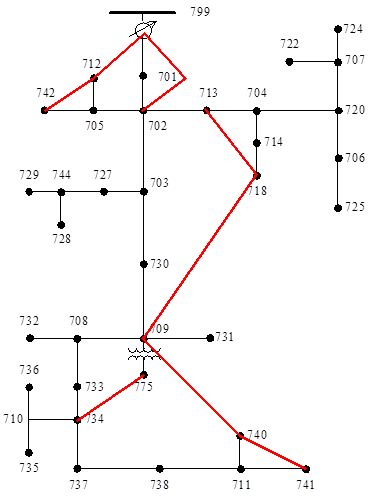
\includegraphics[scale=0.5]{media/ieee_radial_tree_optimized.png}
  \caption{
      IEEE 37 nœuds de test optimisés pour des \textit{prosumer}\newline
      \tiny{Source:\newline
        Smart Grid Topology Designs
      }
  }
  \label{fig:ieee_radial_tree_optimized}
\end{SCfigure}

Cette topologie apporte des réductions de pannes, du trajet de l'énergie et donc de ses pertes énergétiques, pour un coût
minimisé.

Les données des calculs sont disponibles sur le papier Smart Grid Topology Designs de Paula Carroll et Cristina Requejo.